\documentclass[pdflatex,11pt]{aghdpl}
% \documentclass{aghdpl}               % przy kompilacji programem latex
% \documentclass[pdflatex,en]{aghdpl}  % praca w jêzyku angielskim
\usepackage[polish]{babel}
\usepackage{polski}
\usepackage[utf8]{inputenc}

% dodatkowe pakiety
\usepackage{enumerate}
% Listings ------------------------------------------------------------
\usepackage{listings}
% Scala listings
% "define" Scala
\lstdefinelanguage{scala}{
  morekeywords={abstract,case,catch,class,def,%
    do,else,extends,false,final,finally,%
    for,if,implicit,import,match,mixin,%
    new,null,object,override,package,%
    private,protected,requires,return,sealed,%
    super,this,throw,trait,true,try,%
    type,val,var,while,with,yield},
  otherkeywords={=>,<-,<\%,<:,>:,\#,@},
  sensitive=true,
  morecomment=[l]{//},
  morecomment=[n]{/*}{*/},
  morestring=[b]",
  morestring=[b]',
  morestring=[b]"""
}

% IntelliJ Colors for listings
\usepackage{color}
\definecolor{dkgreen}{rgb}{0,0.6,0}
\definecolor{gray}{rgb}{0.5,0.5,0.5}
\definecolor{mauve}{rgb}{0.58,0,0.82}
 
% Default settings for code listings
\lstset{
  frame=tb,
  language=Scala,
  aboveskip=3mm,
  belowskip=3mm,
  showstringspaces=false,
  columns=flexible,
  basicstyle={\small\ttfamily},
  numbers=none,
  numberstyle=\tiny\color{gray},
  keywordstyle=\color{blue},
  commentstyle=\color{gray},
  stringstyle=\color{dkgreen},
  frame=single,
  breaklines=true,
  breakatwhitespace=true
  tabsize=3
}

\lstloadlanguages{TeX}

%---------------------------------------------------------------------------

\author{Konrad Malawski}
\shortauthor{K. Malawski}

\titlePL{ProtoDoc\\Implementacja odpowiednika narzędzia JavaDoc dla jęzka definicji interfejsów Google~Protocol~Buffers}
\titleEN{ProtoDoc\\Development of a JavaDoc tool equivalent for the Google Protocol Buffers Interface~Description~Language}

\shorttitlePL{ProtoDoc - impl. odpowiednika JavaDoc dla Google~Protocol~Buffers} 
\shorttitleEN{ProtoDoc - impl. of JavaDoc like tool for Google~Protocol~Buffers}

\thesistypePL{Praca inżynierska}
\thesistypeEN{Bachelor of Science Thesis}

\supervisorPL{dr inż. Jacek Piwowarczyk}
\supervisorEN{Jacek Piwowarczyk Ph.D}

\date{2011}

\departmentPL{Katedra Automatyki}
\departmentEN{Department of Automatics}

\facultyPL{Wydział Elektrotechniki, Automatyki, Informatyki i Elektroniki}
\facultyEN{Faculty of Electrical Engineering, Automatics, Computer Science and Electronics}

\acknowledgements{TODO podziękowania} % TODO podziękowania

\setlength{\cftsecnumwidth}{10mm}

%---------------------------------------------------------------------------

\begin{document}

\titlepages

\tableofcontents
\clearpage

%---------------------------------------------------------------------------
\chapter{Wprowadzenie}
\label{cha:wprowadzenie}

%---------------------------------------------------------------------------
\section{Cel pracy}
\label{sec:celePracy}


%---------------------------------------------------------------------------
\section{Obecnie dostępne narzędzia}
\label{sec:dostepneNarzedzia}

%===========================================================================
\chapter{Szczegóły implementacyjne}
\label{sec:zastosowanePodejscie}
Jednym z celów projektu jest umożliwienie wykonania parsowania i wygenerowania dokumentacji bez konieczności
instalacji zewnętrznych narzędzi (jakim byłby na przykład \textit{protoc}). Aby sprostać temu wymaganiu konieczna jest implementacja parsera 
języka Protocol Buffers jako części JVM, nie wołając poza nią. Podjęto decyzję wykorzystania \textit{Scala Parser Combinators} (,,kombinatorów parserów'').


%---------------------------------------------------------------------------
\section{Parser}
\subsection{Wprowadzenie do kombinatorów parserów}
TODO klasyfikacja, opisać że są lewo stronnie rekurencyjne etc.

\verb|http://en.wikipedia.org/wiki/Recursive_descent_parser|

\verb|http://en.wikipedia.org/wiki/Left_recursion|
\verb|http://en.wikipedia.org/wiki/Parser_combinator|

\verb|http://stackoverflow.com/questions/17840/how-can-i-learn-about-parser-combinators|

\subsection{Fragmenty implementacji}
Przedstawić fragmenty parsera. Najlepiej go dać jako dodatek jednak w całości.

Parser w tym projekcie budowany jest za pomocą części języka \textit{Scala} zwaną \textit{,,Parser Combinators''}.

\begin{lstlisting}
def messageTypeDef: Parser[ProtoMessageType] = opt(comment) 
                                               ~ "message" ~ ID ~ "{" 
                                               ~ rep(enumTypeDef | instanceField | messageTypeDef) 
                                               ~ "}" ^^ {
  case maybeDoc ~ m ~ id ~ p1 ~ allFields ~ p2 =>
    // utworzenie instancji ProtoMessageType
}
\end{lstlisting}


%---------------------------------------------------------------------------
\section{Verifier}
Generalny opis dlaczego musiał powstac

Przedstawić jakie sprawdzania obsługuję. 
Pokazać że obsługuję importy oraz udowodnić dlaczego konieczny jest dodatkowy krok na to.
No bo bez takiego kroku nie wiedziałbym czy przypadkiem gdzies indziej nie zostal zdefiniowany jakis message etc.

\subsection{Obsługiwane weryfikacje}
Moze sub sectiony o tych checkach oraz konkretne przykłady błędów i jak są komunikowane?


%---------------------------------------------------------------------------
\section{CodeGenerator}
Generator kodu w tym przypadku jest bardzo prostą serią transformacji.
Opisać, wspomnieć że korzystam z mustache etc.

\subsection{Zrzuty ekranu wygenerowanej dokumentacji}
\label{sec:screenshots}

\begin{center}
 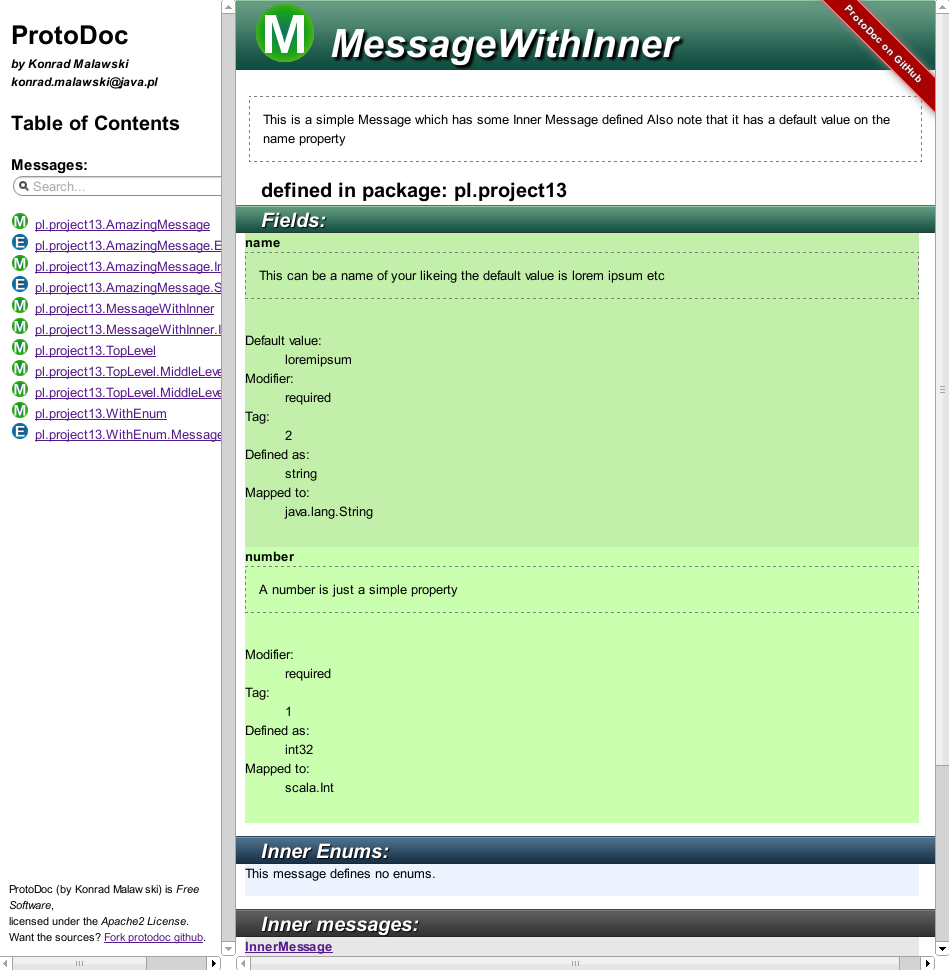
\includegraphics[width=\textwidth]{../protodoc_main.png}
 % protodoc_main.png: 949x970 pixel, 93dpi, 25.92x26.50 cm, bb=0 0 735 751
\end{center}

%===========================================================================
\chapter{Zastosowanie ProtoDoc do automatyzacji dokumentacji projektów}

%===========================================================================
\chapter{Przykład}
Podajemy takie wejście:
\begin{verbatim}
message Person {
  required int32 id = 1;
  required string name = 2;
  optional string email = 3;
}
\end{verbatim}

Następnie wykonanie:

A ostatecznie otrzymujemy taką stronę: \verb|http://protodoc.project13.pl/sample|.

%TODO Tutaj screeny gotowego 


%---------------------------------------------------------------------------
\chapter{Dodatki}
\appendix
\chapter{Podstawy języka Scala}
\label{cha:appendixA}
Celem tego dodatku jest przybliżenie czytelnikowi języka ,,Scala'' aby w wystarczająco płynny sposób mógł czytać przykłady kodu używane w tym dokumencie.

%---------------------------------------------------------------------------
\section{Krótka historia języka}
\label{sec:scala_history}
Język Scala (,,Scalable Language'') najłatwiej jest przedstawić jako hybrydę dwóch znanych nurtów programowania: programowania obiektowego oraz funkcyjnego, wraz z 
powiązanymi z nimi językami programowania. Twórca języka Scala, Martin Oderski\cite{odersky_scala}

Jako konkretnych ,,rodziców'' można by wskazać: 
\begin{itemize}
 \item \textbf{Java} - jako reprezentant nurtu obiektowego 
 \item oraz języki: \textbf{Haskell}, \textbf{SML} oraz pewne elementy języka \textbf{Erlang} (głównie \textit{Actor model}).
\end{itemize}


%---------------------------------------------------------------------------
\section{Podstawy}
\label{sec:scala_basics}
Ta sekcja służy przybliżeniu czyletnikowi języka \textit{Scala} na poziomie wystatczającym aby swobodnie czytać przykłady
kodu umieszczone w tej pracy. W niektórych przykładach pomijane są przypadki skrajne lub nietypowe, celem szybkiego oraz 
jasnego przedstawienia minimum wiedzy na temat języka aby móc swobodnie go ,,czytać''.

\textit{Scala} jest językiem statycznie typowanym posiadającym lokalne ,,Type Inferrence''. Pozwala to kompilatorowi 
\textit{scalac} na ,,odnajdywanie'' typów wszystkich zmiennych oraz typów zwracanych przez metody podczas kompilacji,
bez potrzeby definiowania ich wprost. System ten

Użycie nawiasów \verb|()|, średnika \verb|;| oraz kropki \verb|.| jest analogiczne jak w przypadku Javy, 
jednak w wielu przypadkach opcjonalne gdyż kompilator jest w stanie wydedukować gdzie powinny się znaleźć.
\begin{lstlisting}
 val value = Option(42);
 val other = value.orElse(0);

 // moze zostac zastąpione
 val value = Option(42)
 val other = value orElse 0
\end{lstlisting}

Jednym z ciekawych przykładów stosowania notacji bez nawiasów i kropek jest \textit{ScalaTest}\footnote{ScalaTest - framework do testowania - http://www.scalatest.org}
(przy którego pomocy pisano testy w tym projekcie). Przykładowa \textit{asercja} napisana w \textit{DSL}u definiowanym przez tą bibliotekę wygląda następująco:
\begin{lstlisting}
 messages should (contain key ("Has") and not contain value ("NoSuchMsg"))
\end{lstlisting}



%---------------------------------------------------------------------------
\section{Scala Parser Combinators}
\label{sec:scala_parser_combinators}

\chapter{Podstawy języka Scala oraz Scala Parser Combinators}
\label{cha:appendixB}
Celem tego dodatku jest przybliżenie czytelnikowi języka ,,Scala'' aby w wystarczająco płynny sposób mógł czytać przykłady kodu używane w tym dokumencie.

%---------------------------------------------------------------------------
\section{Krótka historia języka}
\label{sec:scala_history}
Język Scala (,,Scalable Language'') najłatwiej jest przedstawić jako hybrydę dwóch znanych nurtów programowania: programowania obiektowego oraz funkcyjnego, wraz z 
powiązanymi z nimi językami programowania. Twórca języka Scala, Martin Oderski \footnote{Martin Odersky - Strona domowa: \href{http://lamp.epfl.ch/~odersky/}{http://lamp.epfl.ch/~odersky/}}
był ściśle związany z językiem Java - był głównym projektantem generyków w Javie (\textit{Java Generics}) oraz głównym autorem utrzymywanej po dziś dzień
serii kompilatorów \textbf{javac} \footnote{Wywiad z Martinem Odersky na temat korzeni języka Scala - \href{http://www.artima.com/scalazine/articles/origins_of_scala.html}{www.artima.com/.../origins\_of\_scala}}.

Jako konkretnych ,,rodziców'' można by wskazać: 
\begin{itemize}
 \item \textbf{Java} - jako reprezentant nurtu obiektowego 
 \item oraz języki: \textbf{Haskell}, \textbf{SML} oraz pewne elementy języka \textbf{Erlang} (głównie \textit{Actor model}).
\end{itemize}


%---------------------------------------------------------------------------
\section{Podstawy}
\label{sec:scala_basics}
Ta sekcja służy przybliżeniu czyletnikowi języka \textit{Scala} na poziomie wystatczającym aby swobodnie czytać przykłady
kodu umieszczone w tej pracy. W niektórych przykładach pomijane są przypadki skrajne lub nietypowe, celem szybkiego oraz 
jasnego przedstawienia minimum wiedzy na temat języka aby móc swobodnie go ,,czytać''.

\textit{Scala} jest językiem statycznie typowanym posiadającym lokalne ,,Type Inferrence''. Pozwala to kompilatorowi 
\textit{scalac} na ,,odnajdywanie'' typów wszystkich zmiennych oraz typów zwracanych przez metody podczas kompilacji,
bez potrzeby definiowania ich wprost. System ten

Użycie nawiasów \verb|()|, średnika \verb|;| oraz kropki \verb|.| jest analogiczne jak w przypadku Javy, 
jednak w wielu przypadkach opcjonalne gdyż kompilator jest w stanie wydedukować gdzie powinny się znaleźć.
\begin{lstlisting}
 val value = Option(42);
 val other = value.orElse(0);

 // moze zostac zastąpione
 val value = Option(42)
 val other = value orElse 0
\end{lstlisting}

Jednym z ciekawych przykładów stosowania notacji bez nawiasów i kropek jest \textit{ScalaTest}\footnote{ScalaTest - framework do testowania - http://www.scalatest.org}
(przy którego pomocy pisano testy w tym projekcie). Przykładowa \textit{asercja} napisana w \textit{DSL}u definiowanym przez tą bibliotekę wygląda następująco:
\begin{lstlisting}
 messages should (contain key ("Has") and not contain value ("NoSuchMsg"))
\end{lstlisting}

Dostępne jest wiele sposobów definiowania metod / pól w klasie,
w efekcie (na poziomie bytecode), wszystkie przekładane są na wywołania metod. Dostępne są słowa kluczowe:
\begin{itemize}
 \item \textbf{def}, \textit{def}iniujący zwyczajną metodę instancyjną. Warto nadmienić że Javowa koncepcja pojęcia \textit{static} nie jest dostępna z poziomu Scala.
 \item \textbf{val}, deklarujący ,,stałą'' - to jest metodę która raz zawołana, zwróci wartość oraz pole to będzie konsekwentnie zwracać tą samą wartość. 
              Dodatkowym efektem jest traktowanie zmiennych tego typu analogicznie do Javowych zmiennych z modyfikatorem \textbf{final}.
 \item \textbf{var}, deklaruje zwyczajną ,,zmienną'', do jakiej przyzwyczajeni jesteśmy z Java.
 \item modyfikator \textbf{lazy}, wpływający na moment inicjalizacji zmiennej - metody zadeklarowane z modyfikatorem \textbf{lazy} 
       zostaną dopiero zainicjalizowane podczas pierwszego odwołania się do tego pola z innego miejsca w kodzie. 
       W przypadku pary \textbf{lazy val}, metoda ta zostanie zawołana jedynie jednokrotnie, a zwrócona po raz pierwszy wartość
       zostanie zapisana w cache oraz będzie konsekwentnie zwracana podczas ponownych wywołań tej metody.
\end{itemize}

Modyfikator lazy pozwala na eleganckie budowy konstrukcji stosowanych w Parser Combinators, omówionych poniżej.


%---------------------------------------------------------------------------
\section{Traits - wmieszanie zachowania do klasy}
\label{sec:traits}

Słowo kluczowe \textbf{trait} rozpoczyna definicję typu zwanego traitem.
Implementacja nie różni się (na potrzeby tego szybkiego omówienia) od implementowania klasy,
jednak różnica jest podczas ,,dziedziczenia'' przy wykorzystaniu traitów. Nie mówimy bowiem o ,,dziedziczeniu'' 
w przypadku \textit{trait}ów, a o ,,wmieszaniu'' (ang. \textit{mixin} - wmieszanie) zachowania do klasy konkretnej.

Poniżej został przedstawiony najprostrzy trait zawierający jakieś zachowanie, oraz jeden ze sposobów jego wmieszania do klasy konkretnej.
Warto zauważyć że w przypadku wmieszania \textit{trait}a \verb|A| do klasy \verb|Test|, wprowadzamy między nimi relację ,,Test \textbf{IS-A} A'',
analogicznie jak w przypadku dziedziczenia.

\begin{lstlisting}
trait A { 
  def test = "A" // definicja metody zwracającej "A"
}

class Test extends A { } // wmieszanie A

new Test().test // skompiluje i wykona sie poprawnie
\end{lstlisting}

Co ciekawe, nie zauważamy różnicy w przypadku składni odnoszącej się do dziedziczenia dwóch klas konkretnych, oraz wmieszania traita.
Składnia ulega zmianie w przypadku korzystania z więcej niż jeden trait lub domieszania traita do klasy która już dziedziczy po innej klasie,
wówczas zamiast słowa kluczowego \textbf{extends} należy stosować \textbf{with} (nie dozwolone jest wielokrotne zapisanie \textbf{extends},
jednak wielokrotne \textbf{with} są często spotykane). Przykład wmieszania większej ilości traitów zostanie przedstawiony poniżej.

Jest to namiastka dziedziczenia wielobazowego jednak Scala dzięki swojemu bardzo rygorystycznemu kompilatorowi jest w stanie 
uniknąć sytuacji gdzie dziedziczenie wielobazowe byłoby niebezpieczne (klasyczne przykłady 
problematycznych sytuacji w przypadku dziedziczenia wielobazowago można przeczytać w ,,Symfonii C++'', autorstwa pana Grębosza \cite{symfonia}).

Kompilator \textit{scalac} przy napotkaniu konflintów nazw mogących doprowadzić do niejasności ,,którą metodę należy zawołać'', nie skompiluje takiego kodu
oraz poprosi o rozwiązanie konfliktu w sposób explicite. Jako przykład rozważmy dwa \textit{trait}y udostępniające metodę \verb|def test: String|:

\begin{lstlisting}
trait A { def test = "A" }
trait B { def test = "B" }

class Example extends A with B {
  // blad kompilacji!
}
\end{lstlisting}

Przy napotkaniu problemu tego typu kompilator zgłosi:
\begin{verbatim}
error: overriding method test in trait A of type => java.lang.String;
                  method test in trait B of type => java.lang.String needs `override' modifier
class Example extends A with B {
\end{verbatim}

Dzieje się tak ponieważ \textbf{scalac} próbuje odnaleźć która metoda powinna mieć większą wagę, a tymsamym powinna zostać wywołana.
Ponieważ nie jesteśmy w stanie dodać modyfikatora \textbf{override} do żadnego z \textit{trait}ów (ponieważ nie nadpisują one tej metody, a jedynie deklarują),
jedynym możliwym miejscem na rozwiązanie tego konfliktu jest uzupełnienie \verb|Example| o następujący fragment kodu, rutujący poprawnie nasze wywołanie metody:

\begin{lstlisting}
class Example extends A with B {
 // selektywne odwolanie sie do metody konkretnego supertypu
 override def test = super[B].test
}

new Example().test // poprawne
\end{lstlisting}




%---------------------------------------------------------------------------
\section{Scala Parser Combinators}
\label{sec:scala_parser_combinators}


%---------------------------------------------------------------------------
\chapter{Bibliografia}
\bibliographystyle{alpha}
\bibliography{myrefs}

\end{document}
